\documentclass{article}
\usepackage[margin=1in]{geometry}
\usepackage{amsmath,amsthm,amssymb}
\usepackage{bbm,enumerate,mathtools}
\usepackage{tikz,pgfplots}
\usepackage{chessboard}
\usepackage[hidelinks]{hyperref}
\usepackage{multicol} % Problem 35

\newenvironment{question}{\begin{trivlist}\item[\textbf{Question.}]}{\end{trivlist}}
\newenvironment{note}{\begin{trivlist}\item[\textbf{Note.}]}{\end{trivlist}}
\newenvironment{references}{\begin{trivlist}\item[\textbf{References.}]}{\end{trivlist}}
\newenvironment{related}{\begin{trivlist}\item[\textbf{Related.}]\end{trivlist}\begin{enumerate}}{\end{enumerate}}


\begin{document}
  Suppose that there is a ``cop'' and a ``robber'' on an infinite grid, where
  each starts at some given position with some given orientation on the grid,
  and each can move according to some rule set.
  \begin{figure}[ht!]
    \centering
    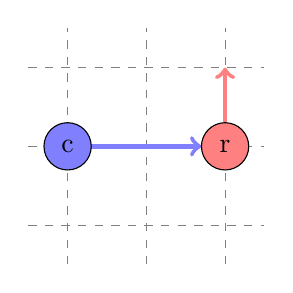
\begin{tikzpicture}
      \draw[gray, dashed] (0.5,0.5) grid (3.5,3.5);
      \draw[ultra thick, ->, blue!50] (1,2)--(2.7,2);
      \draw[fill={blue!50}] (1, 2) circle (0.3cm) node {c};

      \draw[ultra thick, ->, red!50] (3,2)--(3,3);
      \draw[fill={red!50}] (3, 2) circle (0.3cm) node {r};
    \end{tikzpicture}\hspace{1cm}
    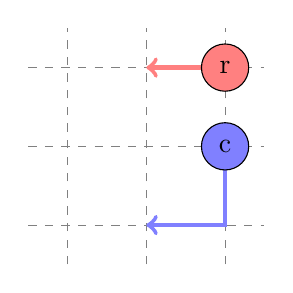
\begin{tikzpicture}
      \draw[gray, dashed] (0.5,0.5) grid (3.5,3.5);
      \draw[ultra thick, ->, blue!50] (3,2)--(3,1)--(2,1);
      \draw[fill={blue!50}] (3, 2) circle (0.3cm) node {c};

      \draw[ultra thick, ->, red!50] (3,3)--(2,3);
      \draw[fill={red!50}] (3, 3) circle (0.3cm) node {r};
    \end{tikzpicture}\hspace{1cm}
    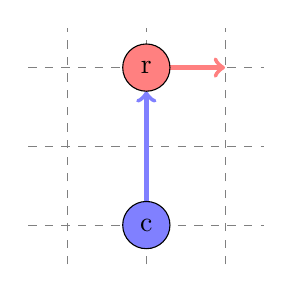
\begin{tikzpicture}
      \draw[gray, dashed] (0.5,0.5) grid (3.5,3.5);
      \draw[ultra thick, ->, blue!50] (2,1)--(2,2.7);
      \draw[fill={blue!50}] (2, 1) circle (0.3cm) node {c};

      \draw[ultra thick, ->, red!50] (2,3)--(3,3);
      \draw[fill={red!50}] (2, 3) circle (0.3cm) node {r};
    \end{tikzpicture}\hspace{1cm}
    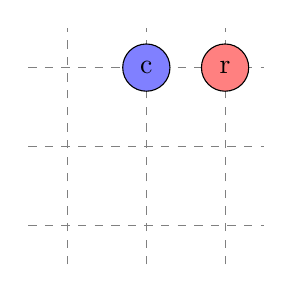
\begin{tikzpicture}
      \draw[gray, dashed] (0.5,0.5) grid (3.5,3.5);
      \draw[fill={blue!50}] (2, 3) circle (0.3cm) node {c};
      \draw[fill={red!50}] (3, 3) circle (0.3cm) node {r};
    \end{tikzpicture}
    \caption{
      In this example, the cop can perform any of the following moves
      $\displaystyle C = \{$
        2 units straight, 1 unit right + 1 unit right, 1 unit right + 1 unit straight
      $\displaystyle\}$
      and the robber can move one unit in any direction along the grid.
      After three steps, the cop has not caught the robber, but if the robber
      moves forward, backward, or right, then she will be caught.
    }
  \end{figure}
\begin{question}
  Is there a procedure for determining in general whether the cop can catch the
  robber?
\end{question}
\begin{related}
  \item Is there a procedure that can put a bound on the number of steps it will
    take for the cop to catch the robber?
  \item If the cop/robber perform moves in their rule set according to some
    distribution, what is the probability that the cop will eventually catch the
    robber?
  \item How does this generalize to a torus, M\"obius strip, cylinder, multiple
    dimensions or a triangular/hexagonal grid?
\end{related}
\end{document}
